\documentclass[11pt,a4paper]{article}

% ------------------------------------------------------------------
% Codificação e idioma
% ------------------------------------------------------------------
\usepackage[utf8]{inputenc}
\usepackage[T1]{fontenc}
\usepackage[brazil]{babel}
\usepackage{lmodern}

% ------------------------------------------------------------------
% Layout e tipografia
% ------------------------------------------------------------------
\usepackage[a4paper,margin=2.3cm]{geometry}
\usepackage{microtype}
\usepackage{setspace}
\onehalfspacing
\usepackage{parskip}
\usepackage{titlesec}
\titleformat{\section}{\large\bfseries\color{azulufpb}}{\thesection}{0.6em}{}
\titleformat{\subsection}{\normalsize\bfseries}{\thesubsection}{0.6em}{}
\titlespacing*{\section}{0pt}{1.4ex plus 1ex minus .2ex}{0.8ex plus .2ex}

% ------------------------------------------------------------------
% Tabelas
% ------------------------------------------------------------------
\usepackage{booktabs}
\usepackage{longtable}
\usepackage{array}
\usepackage{tabularx}
\usepackage{ragged2e}
\newcolumntype{L}[1]{>{\RaggedRight\arraybackslash}p{#1}}
\usepackage{multirow}

% ------------------------------------------------------------------
% Cores e apoio visual
% ------------------------------------------------------------------
\usepackage{graphicx}
\usepackage{float}
\graphicspath{{../../wireframes/}}

\usepackage{xcolor}
\definecolor{azulufpb}{RGB}{31,73,125}
\definecolor{cinzaclaro}{RGB}{242,242,242}
\usepackage[most]{tcolorbox}
\usepackage{enumitem}
\setlist{nosep,leftmargin=1.4em}

% ------------------------------------------------------------------
% Cabeçalho e rodapé
% ------------------------------------------------------------------
\usepackage{fancyhdr}
\pagestyle{fancy}
\fancyhf{}
\lhead{\footnotesize Visualização de Dados (PSAE00218)}
\rhead{\footnotesize Etapa 1 — Descoberta e enquadramento}
\cfoot{\thepage}
\renewcommand{\headrulewidth}{0.3pt}

\usepackage{hyperref}
\hypersetup{colorlinks=true,linkcolor=azulufpb,urlcolor=azulufpb}

% Caixa de destaque para o problema em uma frase
\newtcolorbox{caixadestaque}{colback=cinzaclaro,colframe=azulufpb,
  boxrule=0.8pt,arc=2pt,left=8pt,right=8pt,top=6pt,bottom=6pt}

\begin{document}

% ==================================================================
% CAPA / CABEÇALHO
% ==================================================================
\begin{center}
  {\small UNIVERSIDADE FEDERAL DA PARAÍBA \textbar{} DEPARTAMENTO DE ECONOMIA}\\[2pt]
  {\small Disciplina: Visualização de Dados (PSAE00218) \textbar{} Prof. Jorge Henrique Norões Viana}\\[10pt]
  {\large\bfseries\color{azulufpb} Etapa 1 — Descoberta, Persona e Enquadramento do Problema}\\[4pt]
  {\normalsize Benchmarking regional da produção de cana-de-açúcar na Paraíba}\\[10pt]
  {\small\textbf{Grupo:} Alex Tavares Cordeiro \textbar{} Brenno Henrique Alves da Silva Costa \textbar{} Gustavo Henrique Rocha Oliveira}
\end{center}

\vspace{0.4em}
\hrule
\vspace{1em}

% ==================================================================
% (a) TEMA E CONTEXTO
% ==================================================================
\section{Tema e contexto}

O tema é a produção de cana-de-açúcar na Paraíba, olhada de forma comparativa: como cada
município e a própria Paraíba se posicionam frente a outras regiões produtoras do país, ao
longo das safras. A escolha não é abstrata. A cana é a principal lavoura da Zona da Mata
paraibana e sustenta um conjunto de usinas que decidem, todos os anos, quanto plantar, onde
colher, de quem comprar cana e para onde direcionar a produção entre açúcar e etanol.

O estado atual da informação é fragmentado. Existe dado público e de boa qualidade, mas ele
está espalhado. O IBGE publica a Produção Agrícola Municipal (PAM), com área, produção e
rendimento por município, uma vez por ano. A CONAB acompanha a safra e divulga, por unidade
da federação, a produção de açúcar, de etanol e a qualidade da matéria-prima. A ANP abre os
dados de produção e de venda de etanol. Cada uma dessas fontes vive em um portal diferente,
com formato, calendário e recorte territorial próprios. Quem quer uma leitura comparativa
precisa baixar planilha por planilha e montar a análise à mão.

No setor privado, quem tem estrutura resolve isso pagando. As usinas assinam sistemas de
gestão, consultorias setoriais e boletins que consolidam indicadores. Foi o que apareceu com
clareza na conversa que embasou este projeto: um gerente agrícola relatou que a comparação
entre regiões e a leitura de posicionamento vêm de serviços pagos, e que várias análises
ainda são refeitas manualmente porque o sistema interno não entrega o corte no formato
desejado. A lacuna, então, não é ausência de dado. É ausência de um lugar único, público e
comparável que responda, sem custo de assinatura e sem trabalho manual, onde a produção da
região se posiciona. É essa lacuna que o produto ocupa. Ele não recria os painéis
operacionais de curto prazo que a usina já tem; entrega a leitura comparativa regional que
hoje está dispersa.

% ==================================================================
% (b) PERSONA
% ==================================================================
\section{Persona}

A persona primária foi construída a partir de uma entrevista presencial de aproximadamente
24 minutos com um gerente agrícola de usina em atividade, com áudio gravado e anotações
sintetizadas (roteiro e anotações no anexo). O nome é fictício; o cargo, a rotina e as dores
são os relatados.

\begin{longtable}{L{4.2cm} L{11.2cm}}
\caption{Ficha da persona.}\label{tab:persona}\\
\toprule
\textbf{Campo} & \textbf{Conteúdo}\\
\midrule
\endfirsthead
\toprule
\textbf{Campo} & \textbf{Conteúdo}\\
\midrule
\endhead
\bottomrule
\endfoot
Nome fictício, cargo e formação &
Ricardo Meneses, gerente agrícola. Engenheiro agrônomo formado pela UFPE, cinco anos na
função.\\
\addlinespace
Organização e contexto de trabalho &
Usina sucroalcooleira na Paraíba. Responde por quatro frentes sob sua gestão — agrícola,
transporte e logística, oficina automotiva e segurança do trabalho — e faz interface com os
setores administrativo e industrial.\\
\addlinespace
Decisões que toma na rotina &
Planejamento de plantio, tratos culturais e manejo da colheita (de agosto a março);
planejamento de manutenção de equipamentos e de logística; e contribuição para a definição
do \textit{mix} de produção (açúcar \textit{versus} etanol), decidido a cada safra com base
em preço de mercado.\\
\addlinespace
Frequência e momento de uso do produto &
Uso pontual, ligado ao ciclo da safra: no planejamento anual (o que e onde plantar, de quem
comprar cana) e em revisões antes de reuniões de programação. Não é uso diário; é consulta
estratégica em momentos de decisão.\\
\addlinespace
Letramento em dados &
Alto. Trabalha com relatórios, tabelas dinâmicas e painéis de Power BI; interpreta gráficos
comparativos de orçamento, custo e metas; e refaz análises em Excel quando o sistema não
entrega o corte desejado.\\
\addlinespace
Ferramentas e fontes que já utiliza &
Sistema integrado de gestão (pago), Power BI, Excel, sistema de monitoramento de frota e de
RH; boletins setoriais estaduais (quinzenais) e nacionais (semanais), ambos por assinatura.\\
\addlinespace
O que hoje a impede de decidir bem &
A informação comparativa entre regiões está dispersa em fontes separadas e, em boa parte,
paga. Análises relevantes são refeitas manualmente porque o sistema não automatiza o corte.
Não há um lugar único e público que mostre o posicionamento da região frente ao país.\\
\addlinespace
Evidência que sustenta esta ficha &
Entrevista presencial de $\approx$24 min com gerente agrícola em atividade, áudio gravado e
anotações sintetizadas (anexo). Trechos-chave: ``todos os sistemas são pagos''; relato de
análises refeitas à mão; decisão de \textit{mix} guiada por preço de mercado.\\
\end{longtable}

% ==================================================================
% (c) JORNADA DE DECISÃO
% ==================================================================
\section{Jornada de decisão}

O mapa abaixo descreve como Ricardo chega hoje a uma decisão de posicionamento regional —
por exemplo, avaliar se vale expandir área ou de quais fornecedores de cana se aproximar —
sem o produto proposto.

\begin{longtable}{L{3.4cm} L{4.3cm} L{3.6cm} L{3.6cm}}
\caption{Jornada de decisão da persona.}\label{tab:jornada}\\
\toprule
\textbf{Momento} & \textbf{O que a persona faz hoje} & \textbf{Ponto de dor} & \textbf{Oportunidade para o produto}\\
\midrule
\endfirsthead
\toprule
\textbf{Momento} & \textbf{O que a persona faz hoje} & \textbf{Ponto de dor} & \textbf{Oportunidade para o produto}\\
\midrule
\endhead
\bottomrule
\endfoot
Percebe a necessidade &
Antes do planejamento de safra, precisa entender como a produtividade da região evoluiu e
como se compara à de outras. &
A pergunta é clara, mas a resposta exige juntar fontes que não conversam. &
Abrir uma tela única que já mostre o posicionamento da região no país.\\
\addlinespace
Busca a informação &
Recorre ao sistema interno, a boletins pagos e a planilhas próprias; parte vem de consultoria
por assinatura. &
Fontes separadas, com custo e calendários diferentes. &
Centralizar dado público (IBGE, CONAB, ANP) num só lugar, sem assinatura.\\
\addlinespace
Organiza e compara &
Exporta números e monta a comparação manualmente em Excel, alinhando períodos e recortes. &
Retrabalho manual; o sistema não entrega o corte pronto. &
Comparação automática entre municípios, estados e safras, com indicadores já calculados.\\
\addlinespace
Interpreta &
Lê os números à luz da experiência e cruza com a leitura de mercado. &
Falta referência explícita (média regional, período anterior) ao lado do número. &
Mostrar cada valor junto de sua referência de comparação.\\
\addlinespace
Decide e age &
Define prioridades de plantio, área e relação com fornecedores. &
A decisão carrega incerteza sobre o posicionamento relativo da região. &
Sustentar a decisão com o benchmarking regional visível e atualizado.\\
\end{longtable}

% ==================================================================
% (d) ENQUADRAMENTOS ALTERNATIVOS
% ==================================================================
\section{Enquadramentos alternativos}

A partir do mesmo ponto de dor — a informação comparativa está dispersa e é cara —, três
enquadramentos foram formulados. Eles apontam para produtos genuinamente diferentes.

\begin{longtable}{c L{5.0cm} L{4.4cm} L{4.4cm}}
\caption{Enquadramentos considerados e escolha.}\label{tab:enquadramentos}\\
\toprule
\textbf{\#} & \textbf{Enquadramento (``Como poderíamos...?'')} & \textbf{Produto que resultaria} & \textbf{Por que foi ou não escolhido}\\
\midrule
\endfirsthead
\toprule
\textbf{\#} & \textbf{Enquadramento} & \textbf{Produto que resultaria} & \textbf{Por que foi ou não escolhido}\\
\midrule
\endhead
\bottomrule
\endfoot
1 &
Como poderíamos ajudar o gestor a situar a produção da sua região frente às demais regiões
produtoras do país? &
Painel de benchmarking regional de produtividade, por município, estado e safra. &
\textbf{Escolhido.} Usa dado público municipal, casa com a cadência anual da decisão e ocupa
a lacuna comparativa que hoje é paga e manual.\\
\addlinespace
2 &
Como poderíamos antecipar ao gestor a melhor divisão entre açúcar e etanol na próxima safra? &
Ferramenta de recomendação de \textit{mix} guiada por preço de mercado. &
Não escolhido. Depende de preço internacional em tempo quase real, que não é público
municipal e recai sobre a área comercial, não a agrícola.\\
\addlinespace
3 &
Como poderíamos consolidar os indicadores operacionais internos da usina num painel único? &
Painel operacional interno (frota, oficina, ordens de serviço, metas). &
Não escolhido. Duplicaria sistemas que a usina já tem e dependeria de dados internos,
privados, fora do escopo público exigido.\\
\end{longtable}

A escolha do enquadramento 1 se justifica em três frentes. É \textbf{relevante para a
persona}, porque responde a uma pergunta que ela hoje resolve com esforço e custo. É
\textbf{viável com os dados disponíveis}, porque o IBGE entrega produtividade em nível
municipal e a CONAB entrega a camada industrial por estado, ambos confirmados por coleta
direta. E tem \textbf{potencial de gerar ação}, porque o posicionamento relativo alimenta
decisões concretas de plantio, área e relação com fornecedores.

% ==================================================================
% (e) PROBLEMA E PERGUNTA DE DECISÃO
% ==================================================================
\section{Problema e pergunta de decisão}

\begin{caixadestaque}
Ricardo, gerente agrícola de usina na Paraíba, precisa situar a produtividade da sua região
frente a outras regiões produtoras para decidir plantio, área e relação com fornecedores, mas
a informação comparativa está dispersa em fontes separadas e pagas e é montada à mão, o que
faz a decisão depender de leitura fragmentada e de retrabalho manual.
\end{caixadestaque}

\textbf{Pergunta de decisão principal:} \textit{como a produtividade e a produção de
cana-de-açúcar da minha região se comparam às de outras regiões do país, e como esse
posicionamento evoluiu ao longo das safras?} É a pergunta que o produto responde toda vez que
é aberto. É específica o bastante para admitir resposta com os dados em mãos e ampla o
bastante para justificar filtros por região, período e indicador — logo, um produto
interativo em vez de um número solto.

% ==================================================================
% (f) CRITÉRIOS DE SUCESSO
% ==================================================================
\section{Critérios de sucesso}

Antes de construir, declaramos como saberemos que a persona foi ajudada:

\begin{itemize}
  \item \textbf{Tempo.} O levantamento comparativo que hoje é feito abrindo várias fontes e
  montando planilha à mão passa a ser resolvido em uma consulta de poucos minutos.
  \item \textbf{Comportamento.} A persona passa a consultar o produto antes das reuniões de
  planejamento de safra, em vez de recorrer apenas a boletins pagos.
  \item \textbf{Decisão.} O posicionamento da região deixa de ser lido ``de memória'' e passa
  a ser sustentado por um número com referência explícita de comparação.
  \item \textbf{Custo.} Parte da leitura comparativa hoje obtida por assinatura passa a ser
  coberta por fonte pública, reduzindo dependência de serviço pago.
\end{itemize}

Esses critérios serão retomados na Etapa 3 para avaliar honestamente o resultado.

% ==================================================================
% (g) PERGUNTAS ANALÍTICAS
% ==================================================================
\section{Perguntas analíticas}

As perguntas abaixo, da mais geral à mais específica, formam o esqueleto do painel das
etapas seguintes.

\begin{longtable}{c L{4.6cm} L{3.4cm} L{2.6cm} L{2.8cm}}
\caption{Perguntas analíticas, indicadores e forma visual.}\label{tab:perguntas}\\
\toprule
\textbf{\#} & \textbf{Pergunta analítica} & \textbf{Indicador(es)} & \textbf{Tipo de comparação} & \textbf{Visual pretendido}\\
\midrule
\endfirsthead
\toprule
\textbf{\#} & \textbf{Pergunta analítica} & \textbf{Indicador(es)} & \textbf{Comparação} & \textbf{Visual}\\
\midrule
\endhead
\bottomrule
\endfoot
1 & Como está distribuída a produção de cana entre as regiões do país? & Quantidade produzida; participação regional (\%) & Composição / posição no espaço & Mapa coroplético e barras\\
\addlinespace
2 & Como a produtividade da região evoluiu ao longo das safras? & Produtividade (t/ha) & Evolução & Linha temporal\\
\addlinespace
3 & Como a produtividade da região se compara à de outras, na mesma escala? & Produtividade (t/ha) frente à referência regional & Desvio em relação a referência & Barras divergentes\\
\addlinespace
4 & Quais microrregiões vêm ganhando ou perdendo produtividade de forma consistente? & Tendência de produtividade (t/ha por ano) & Evolução / ranqueamento & Barras ordenadas\\
\addlinespace
5 & Como se divide o destino da cana entre açúcar e etanol na região? & \textit{Mix} açúcar/etanol; ATR (kg/t) & Composição & Barras empilhadas\\
\end{longtable}

% ==================================================================
% (h) DADOS
% ==================================================================
\section{Dados}

O produto se apoia em três fontes públicas, todas coletadas diretamente durante a fase de
descoberta (os \textit{scripts} de coleta e as amostras acompanham a entrega).

\begin{itemize}
  \item \textbf{IBGE — Produção Agrícola Municipal (Tabela 1612 do SIDRA).} Fonte principal.
  Traz área plantada, área colhida, quantidade produzida, rendimento médio e valor da produção
  da cana-de-açúcar (produto 2696). Recorte temporal anual, de 1974 a 2025; recorte geográfico
  do Brasil ao município. Coletada via API pública, sem cadastro. Volume: a consulta abrange os
  223 municípios da Paraíba, embora apenas cerca de 120 apresentem produção de cana registrada
  em algum ano (os demais vêm suprimidos, ver limitações), e a consulta nacional cobre as 27
  unidades da federação.
  \item \textbf{CONAB — Série Histórica da Cana.} Camada industrial. Traz produção de açúcar,
  de etanol (anidro, hidratado e total) e o ATR por unidade da federação e safra, de 2005/06
  em diante. Arquivo aberto em texto; 470 registros, dos quais 22 safras da Paraíba.
  \item \textbf{ANP — dados abertos de etanol.} Contexto de demanda e produção industrial.
  Vendas anuais de etanol hidratado por município (1990–2024; 5.079 registros da Paraíba, 348
  municípios, com código IBGE) e produção de etanol por unidade da federação (mensal, desde
  2012). Arquivos CSV abertos.
\end{itemize}

Condições de uso: as três são de acesso público e livre, sem necessidade de cadastro,
divulgadas pelos respectivos órgãos oficiais. O dicionário abaixo reúne as variáveis centrais.

\begin{longtable}{L{3.4cm} L{5.4cm} L{1.8cm} L{2.0cm} L{2.4cm}}
\caption{Dicionário de dados.}\label{tab:dicionario}\\
\toprule
\textbf{Variável} & \textbf{Descrição} & \textbf{Tipo} & \textbf{Unidade} & \textbf{Fonte e período}\\
\midrule
\endfirsthead
\toprule
\textbf{Variável} & \textbf{Descrição} & \textbf{Tipo} & \textbf{Unidade} & \textbf{Fonte e período}\\
\midrule
\endhead
\bottomrule
\endfoot
Quantidade produzida & Massa de cana colhida no território no ano & Numérico & toneladas & IBGE PAM, 1974–2025\\
\addlinespace
Área colhida & Área efetivamente colhida de cana & Numérico & hectares & IBGE PAM, 1974–2025\\
\addlinespace
Rendimento médio & Produção por unidade de área (publicado pelo IBGE) & Numérico & kg/ha & IBGE PAM, 1974–2025\\
\addlinespace
Valor da produção & Valor da produção agrícola de cana & Numérico & mil reais & IBGE PAM, 1994–2025\\
\addlinespace
Produção de açúcar & Açúcar produzido pela indústria na UF/safra & Numérico & mil t & CONAB, 2005/06–\\
\addlinespace
Produção de etanol total & Etanol (anidro + hidratado) na UF/safra & Numérico & mil L & CONAB, 2005/06–\\
\addlinespace
ATR & Açúcar total recuperável por tonelada de cana & Numérico & kg/t & CONAB, 2005/06–\\
\addlinespace
Vendas de etanol hidratado & Volume de etanol hidratado vendido no município & Numérico & litros & ANP, 1990–2024\\
\addlinespace
Código do município (IBGE) & Identificador do município, chave de junção & Categórico & --- & ANP / IBGE\\
\end{longtable}

\textbf{Três limitações conhecidas da base:}
\begin{enumerate}
  \item \textbf{Supressão em municípios pequenos.} Na PAM, municípios de produção muito baixa
  retornam valor ausente (``-''). Uma verificação preliminar mostrou que cerca de 62\% dos
  registros municipais-ano de rendimento estão suprimidos, contra 36\% no nível de microrregião
  e nenhum no de UF. Por isso a análise de série de longo prazo trabalha na microrregião, e o
  município fica reservado ao retrato de um único ano.
  \item \textbf{Calendários diferentes.} O IBGE trabalha em ano civil e a CONAB em safra (ano
  agrícola). Cruzar as duas exige uma regra declarada de alinhamento temporal.
  \item \textbf{Granularidade e defasagem.} A camada industrial (açúcar, etanol, ATR) só
  existe em nível estadual, não municipal; e a PAM fecha com cerca de um ano de atraso,
  enquanto a CONAB divulga estimativas por levantamento antes do número consolidado.
\end{enumerate}

% ==================================================================
% (i) INDICADORES DERIVADOS
% ==================================================================
\section{Indicadores derivados}

Os indicadores abaixo são calculados a partir das variáveis brutas, não lidos prontos. A
fórmula da produtividade foi validada na fase de descoberta: recompor o rendimento a partir de
quantidade e área colhida reproduz exatamente o rendimento publicado pelo IBGE. Uma ressalva de
método já confirmada: a produtividade não é aditiva, logo é calculada como soma de quantidade
sobre soma de área, nunca como média de rendimentos.

\begin{enumerate}
  \item \textbf{Produtividade da cana.}
  \\ Fórmula: quantidade produzida (t) $\div$ área colhida (ha).
  \\ Unidade: t/ha. \quad Sentido: maior é melhor.
  \\ Referência: média da microrregião, média estadual, média nacional e safra anterior.

  \item \textbf{Participação regional na produção.}
  \\ Fórmula: produção da unidade $\div$ produção do agregado (estado ou Brasil) $\times$ 100.
  \\ Unidade: \%. \quad Sentido: contextual (mede peso e concentração).
  \\ Referência: total estadual ou nacional.

  \item \textbf{Tendência de produtividade.}
  \\ Fórmula: inclinação da reta ajustada à série de produtividade, em janela recente.
  \\ Unidade: t/ha por ano. \quad Sentido: positivo é melhor.
  \\ Referência: zero (estável) e a tendência das demais regiões da mesma escala.

  \item \textbf{Mix açúcar/etanol.}
  \\ Fórmula: relação entre etanol (mil L) e açúcar (mil t) produzidos na safra, lida junto do
  ATR (kg/t).
  \\ Unidade: proporção. \quad Sentido: contextual (decisão estratégica).
  \\ Referência: média nacional e safra anterior.
\end{enumerate}

A comparação de produtividade contra uma referência (o desvio percentual frente à média do
grupo) permanece disponível como forma de leitura, não como indicador autônomo, por ser uma
transformação direta da própria produtividade.

% ==================================================================
% (j) MENSAGEM CENTRAL E AÇÕES ESPERADAS
% ==================================================================
\section{Mensagem central e ações esperadas}

\textbf{Mensagem central:} \textit{a produtividade da sua região tem um lugar definido no
mapa nacional da cana, e esse lugar pode ser visto, comparado e acompanhado safra a safra sem
depender de serviço pago.}

A partir dessa leitura, a persona deve poder:
\begin{itemize}
  \item \textbf{Priorizar área e plantio}, direcionando esforço para onde a produtividade
  relativa indica maior retorno.
  \item \textbf{Reavaliar a relação com fornecedores de cana}, comparando o desempenho de
  municípios de origem.
  \item \textbf{Revisar metas de safra} com base no posicionamento frente à média regional e
  nacional, e não apenas na série interna.
\end{itemize}

% ==================================================================
% (k) ESBOÇO DE BAIXA FIDELIDADE
% ==================================================================
\section{Esboço de baixa fidelidade}\label{sec:esboco}

Foram produzidos três esboços da tela principal antes de escolher um para detalhar. Os três
partem da mesma pergunta de decisão, mas organizam a resposta de formas diferentes.

\begin{itemize}
  \item \textbf{Esboço A — mapa em primeiro plano.} O mapa coroplético do país ocupa o centro,
  com a Paraíba destacada; filtros à esquerda e indicadores-resumo no topo.
  \item \textbf{Esboço B — comparação em primeiro plano.} Barras divergentes de desvio de
  produtividade dominam a tela; o mapa vira apoio lateral.
  \item \textbf{Esboço C — evolução em primeiro plano.} A série temporal do rendimento abre a
  tela, com o \textit{ranking} de municípios logo abaixo.
\end{itemize}

\textbf{Escolha: esboço A.} Ele responde primeiro à pergunta de posicionamento (``onde minha
região está''), que é a mais geral, e deixa evolução e ranking como aprofundamento.

\begin{figure}[H]
  \centering
  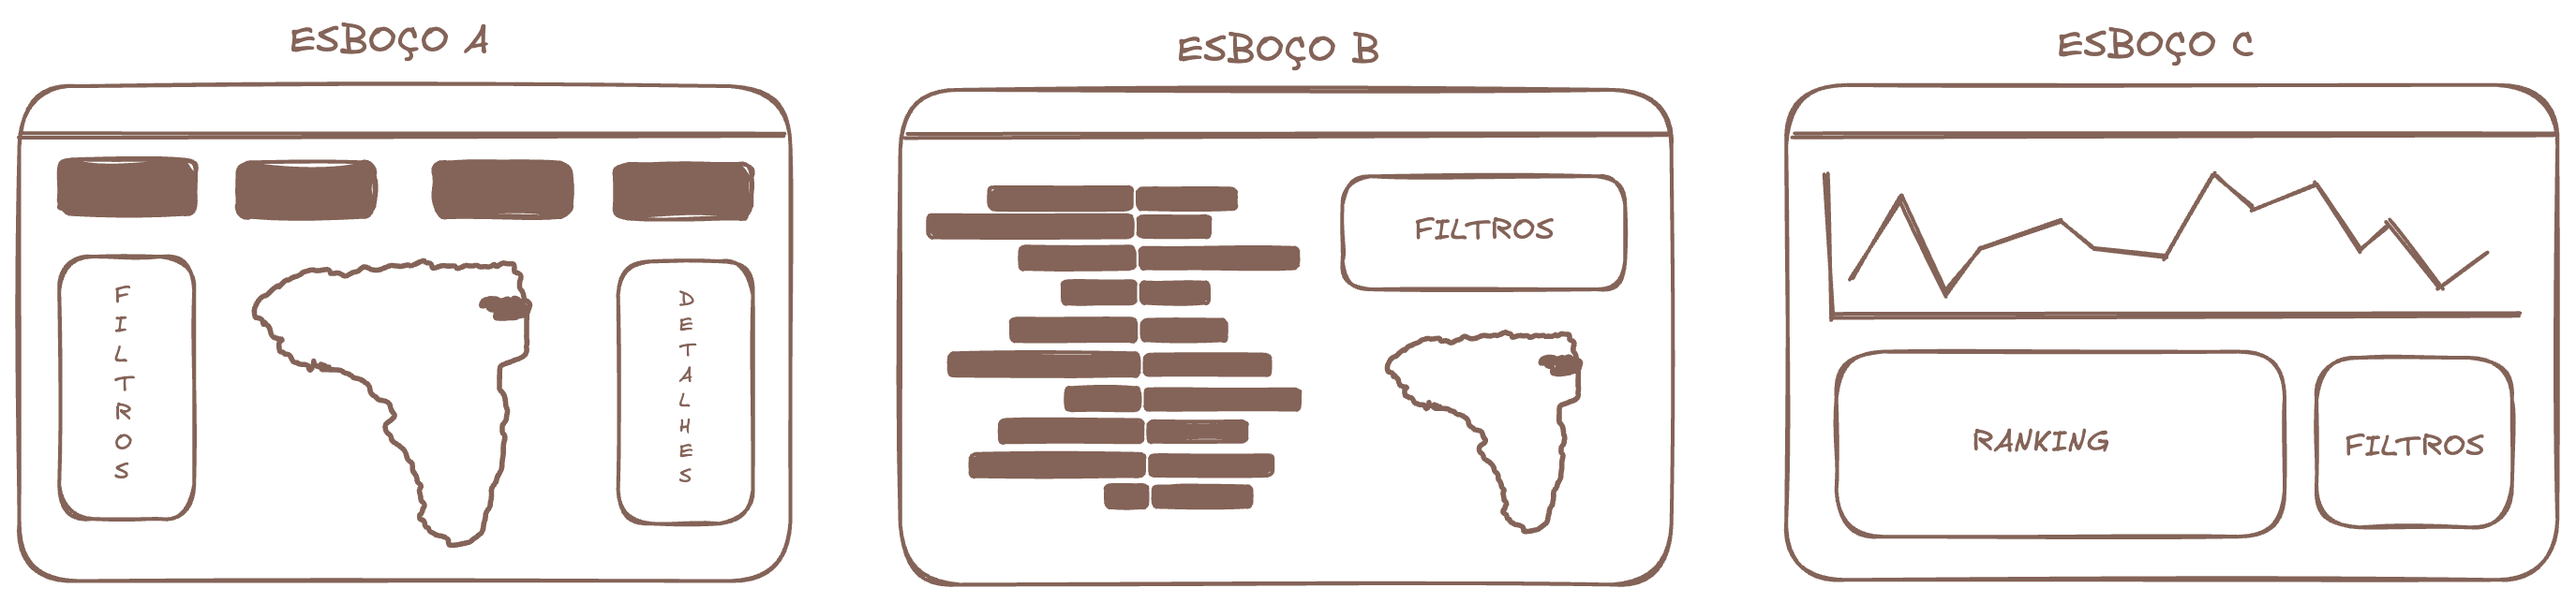
\includegraphics[width=\textwidth]{esbocos-sem-fundo.png}
  \caption{Três esboços de baixa fidelidade da tela principal. Da esquerda para a direita:
  esboço A (mapa em primeiro plano), esboço B (comparação em primeiro plano) e esboço C
  (evolução em primeiro plano). Sem cores definitivas, dados reais ou logotipos.}
  \label{fig:esbocos}
\end{figure}

A partir do esboço A escolhido, foi detalhado o fluxo completo de navegação, feito no Figma,
sem cores definitivas, sem dados reais e sem logotipos, indicando o que fica acima da dobra,
onde ficam os filtros, onde fica a mensagem principal, o que é clicável e o que é apenas
informativo. As três telas do fluxo são apresentadas a seguir.

\begin{figure}[H]
  \centering
  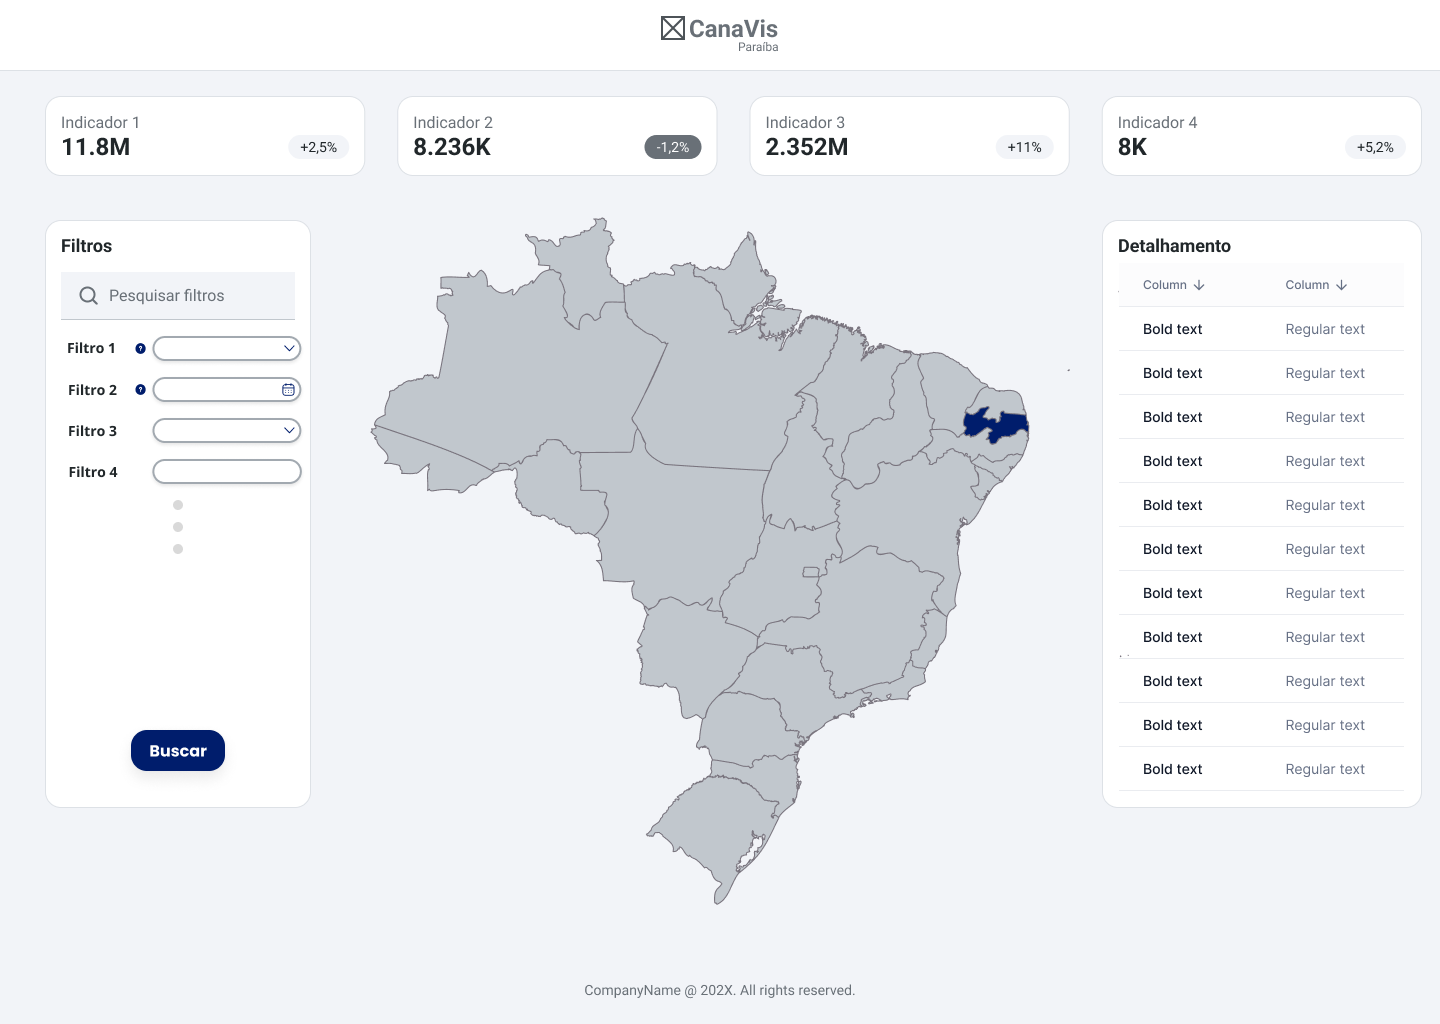
\includegraphics[width=\textwidth]{tela-inicial.png}
  \caption{Tela inicial — panorama nacional. Situa a região no mapa da produção do país; é o
  ponto de entrada do produto.}
  \label{fig:tela-inicial}
\end{figure}

\begin{figure}[H]
  \centering
  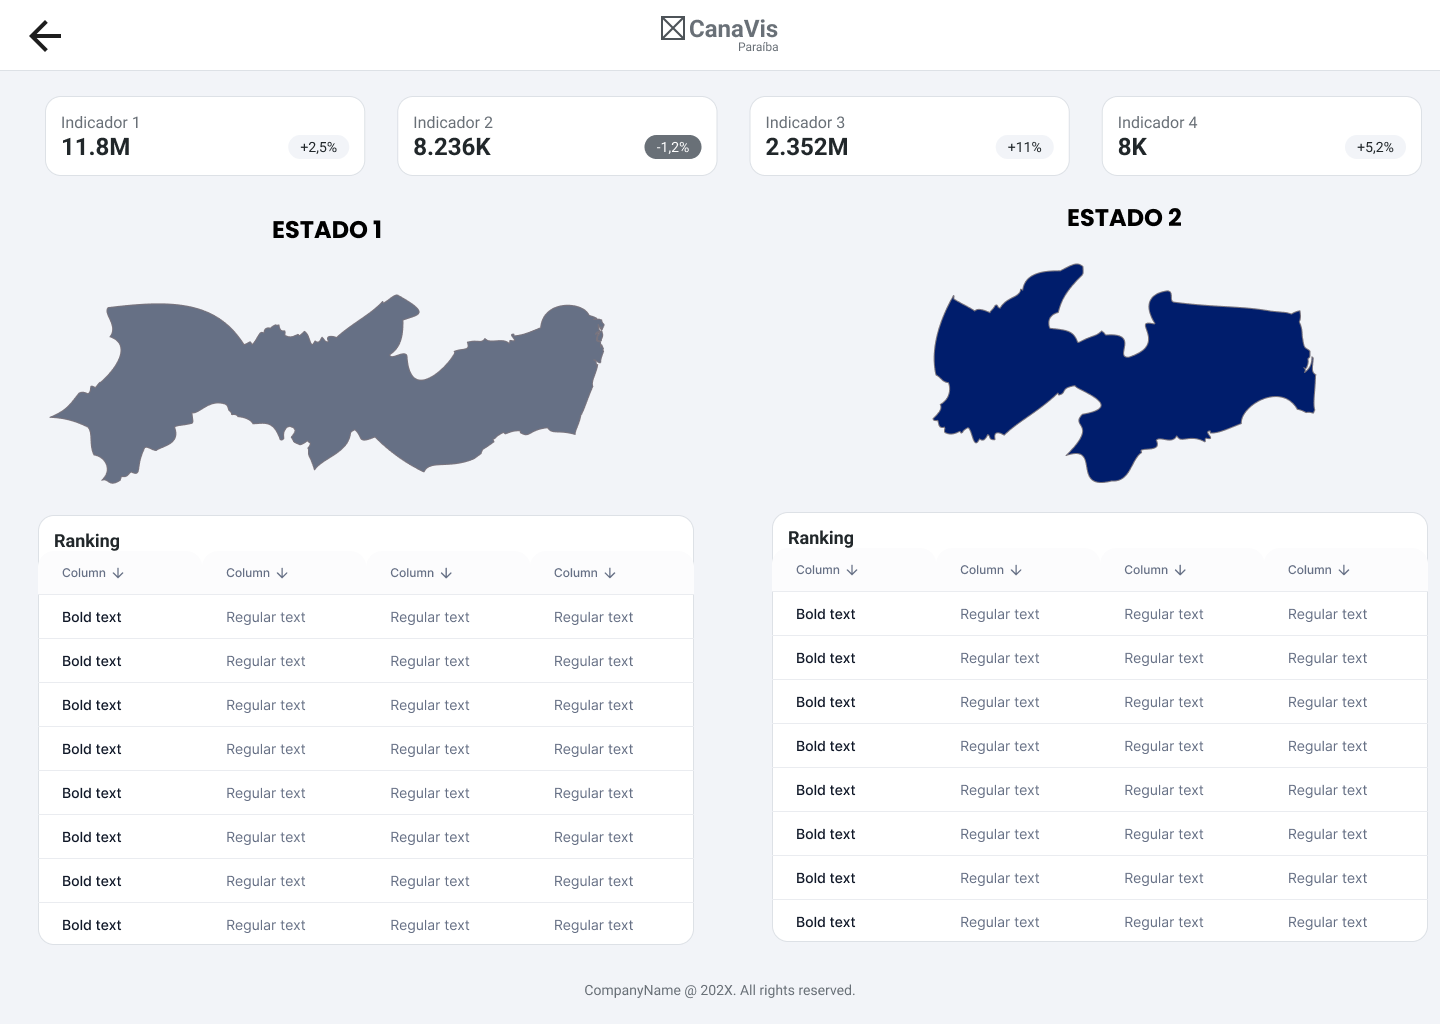
\includegraphics[width=\textwidth]{tela-estado.png}
  \caption{Segunda tela — detalhe do estado. Mostra a evolução e o \textit{ranking} de
  municípios da UF selecionada no panorama nacional.}
  \label{fig:tela-estado}
\end{figure}

\begin{figure}[H]
  \centering
  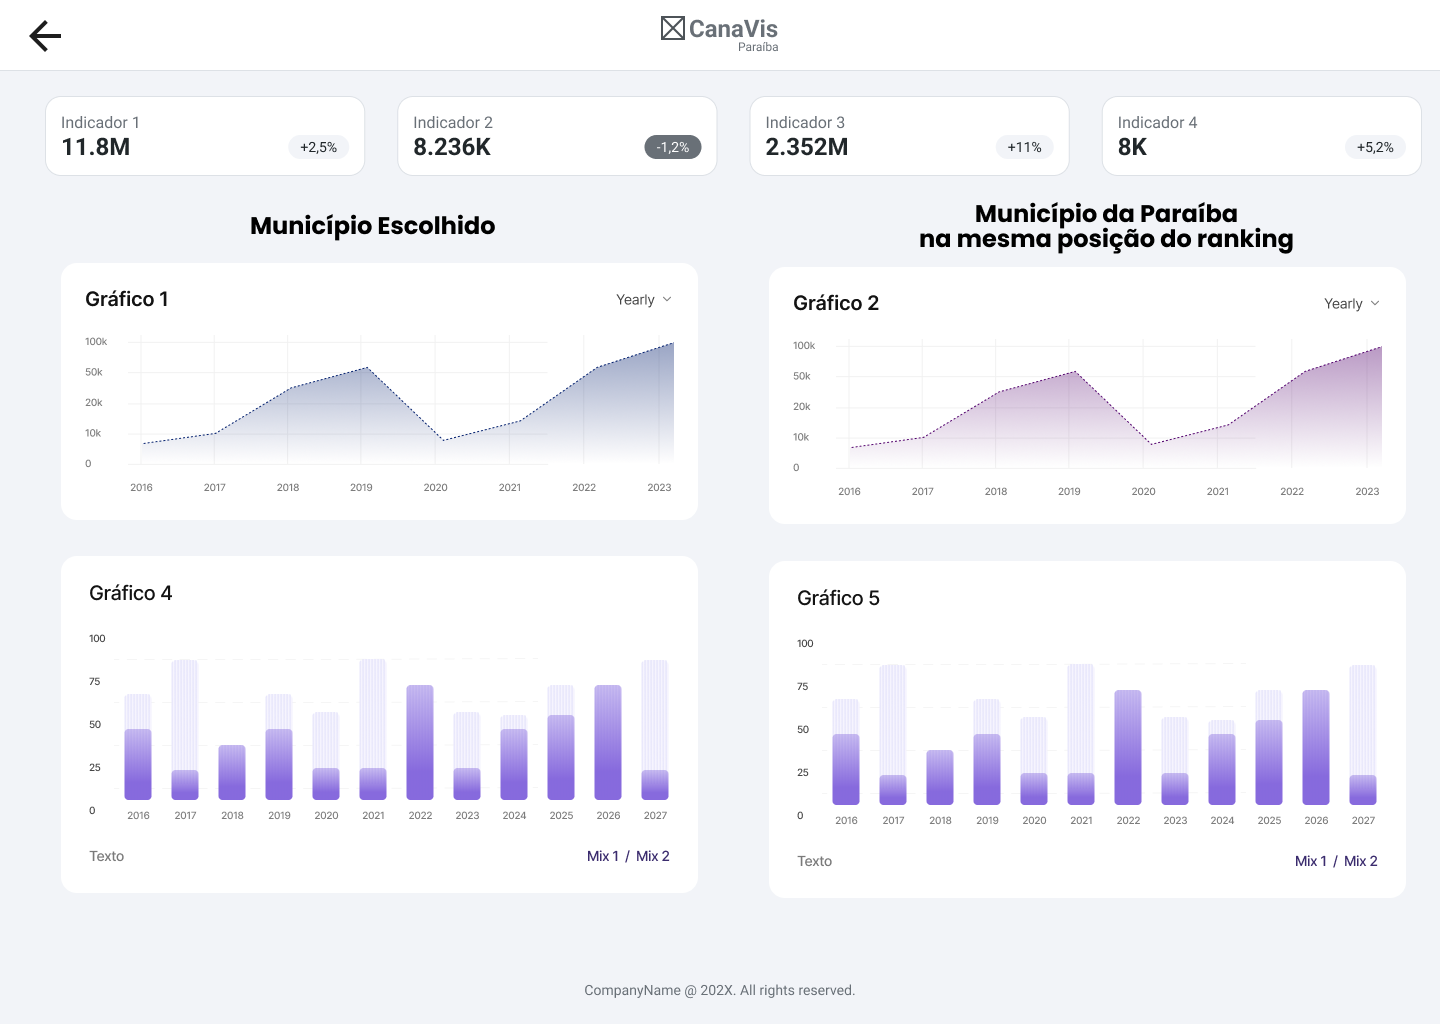
\includegraphics[width=\textwidth]{tela-municipio.png}
  \caption{Terceira tela — detalhe do município. Aprofunda a série histórica e o \textit{mix}
  açúcar/etanol de um município específico.}
  \label{fig:tela-municipio}
\end{figure}

% ==================================================================
% (l) MAPA DE NAVEGAÇÃO
% ==================================================================
\section{Mapa de navegação}

\begin{longtable}{L{2.8cm} L{4.0cm} L{2.6cm} L{2.6cm} L{2.6cm}}
\caption{Mapa de navegação previsto.}\label{tab:navegacao}\\
\toprule
\textbf{Tela} & \textbf{Objetivo da tela} & \textbf{Chega a partir de} & \textbf{Leva para} & \textbf{Gatilho da transição}\\
\midrule
\endfirsthead
\toprule
\textbf{Tela} & \textbf{Objetivo} & \textbf{Chega de} & \textbf{Leva para} & \textbf{Gatilho}\\
\midrule
\endhead
\bottomrule
\endfoot
Panorama nacional & Situar a região no mapa da produção do país & Abertura & Detalhe do estado & Clique em um estado no mapa\\
\addlinespace
Detalhe do estado & Mostrar evolução e ranking de municípios da UF & Panorama nacional & Detalhe do município & Clique em um município\\
\addlinespace
Detalhe do município & Aprofundar a série e o mix de um município & Detalhe do estado & Panorama nacional & Botão de voltar / seleção de nova UF\\
\end{longtable}

As três telas do mapa acima correspondem, na ordem, aos esboços detalhados da
Seção~\ref{sec:esboco}: o \textbf{panorama nacional} é a tela inicial
(Figura~\ref{fig:tela-inicial}); o \textbf{detalhe do estado} é a segunda tela
(Figura~\ref{fig:tela-estado}), alcançada ao clicar em um estado no mapa; e o
\textbf{detalhe do município} é a terceira tela (Figura~\ref{fig:tela-municipio}), alcançada
ao clicar em um município do \textit{ranking}. A mudança de rota entre essas telas é o
compromisso que será cobrado nas Etapas 2 e 3.

% ==================================================================
% (m) RISCOS ÉTICOS E DE INTERPRETAÇÃO
% ==================================================================
\section{Riscos éticos e de interpretação}

O maior risco é o \textbf{ranking mal lido}. Ao ordenar municípios por produtividade, é fácil
concluir que um município ``é pior'' quando, na verdade, ele tem área pequena, produção
suprimida na base, ou condições agronômicas distintas. Municípios e produtores podem ser
prejudicados por uma leitura apressada que os coloque no fim de uma lista sem contexto.

Salvaguardas adotadas:
\begin{itemize}
  \item \textbf{Denominadores explícitos.} Toda produtividade aparece com a área colhida que a
  originou, para que o leitor veja a escala por trás do número.
  \item \textbf{Tratamento visível dos ausentes.} Municípios com dado suprimido são marcados
  como ``sem informação'', nunca como zero, para não distorcer médias e rankings.
  \item \textbf{Referência ao lado do número.} Nenhum valor aparece sozinho; sempre acompanha
  a média de comparação e o período.
  \item \textbf{Recusa de recortes frágeis.} Comparações entre anos de metodologias ou
  calendários diferentes (ano civil do IBGE \textit{versus} safra da CONAB) só aparecem quando
  o alinhamento temporal está declarado.
\end{itemize}

% ==================================================================
% DISCUSSÃO
% ==================================================================
\section{Discussão}

\textbf{Por que um produto interativo, e não um relatório estático?} Porque a pergunta muda a
cada uso. Ora interessa comparar a Paraíba com o Nordeste, ora comparar dois municípios, ora
olhar a evolução de uma safra específica. Um relatório fixo responderia a um recorte e
envelheceria; o produto interativo deixa a persona escolher o recorte que a decisão do momento
exige, com o dado sempre atualizado na fonte.

\textbf{Uma validação preliminar já foi feita.} Embora esta etapa trate de enquadramento, o
grupo adiantou uma checagem estatística dos indicadores sobre os dados reais, registrada no
repositório do projeto (notebooks de análise e registros de decisão). Dessa checagem vieram
três ajustes já incorporados acima: a produtividade é tratada como medida não aditiva; o desvio
frente à referência deixou de ser indicador autônomo por ser transformação direta da
produtividade; e a análise de longo prazo foi fixada no nível de microrregião, dada a
supressão municipal. Um indicador de resiliência climática foi considerado, mas o cruzamento
com dados públicos de chuva não sustentou relação estatística na faixa canavieira, e a
investigação ficou documentada para retomada futura.

\textbf{O que ainda está incerto e será decidido na Etapa 2?} A regra de alinhamento entre ano
civil (IBGE) e safra (CONAB), que precisa ser testada antes de virar medida, e a forma final de
comparar regiões de escalas muito diferentes sem que o ranking vire ranking de porte.

\textbf{O que faríamos diferente com o dobro do tempo?} Investiríamos em incorporar o Comex
Stat, hoje deixado de fora porque sua API está protegida por verificação anti-robô, e o
emprego setorial do CAGED. Eles enriqueceriam a leitura da cadeia — destino da produção e peso
socioeconômico —, mas não são essenciais para responder à pergunta de decisão principal, e por
isso ficaram fora do escopo desta etapa.

% ==================================================================
% ANEXO
% ==================================================================
\newpage
\section*{Anexo — Pesquisa com a persona}
\addcontentsline{toc}{section}{Anexo}

\textbf{Formato:} entrevista presencial de aproximadamente 24 minutos com gerente agrícola de
usina em atividade, com áudio gravado e anotações sintetizadas. O roteiro seguiu quatro blocos:
contexto e decisões; caminho da informação e dificuldades; comparações, uso e interpretação;
e teste da hipótese.

\textbf{Roteiro de perguntas (resumo):}
\begin{enumerate}
  \item Formação e responsabilidades atuais na usina.
  \item Decisões agrícolas que toma e em que momentos.
  \item Situação recente de decisão com uso de dados de produção.
  \item Caminho da necessidade de informação até a decisão (sistemas, planilhas, pessoas).
  \item Uso de informações de fora da usina e verificação de confiança.
  \item Maior dificuldade no processo.
  \item Comparações de produção úteis hoje (períodos, áreas, territórios).
  \item Momento da rotina em que a consulta externa faria diferença.
  \item Como interpreta tabelas e gráficos e verifica se a comparação é válida.
  \item Situação concreta em que a consulta proposta ajudaria.
  \item Necessidade prioritária e como perceberia melhora.
  \item Confirmação da síntese do problema.
\end{enumerate}

\textbf{Anotações sintetizadas (pontos-chave relatados):}
\begin{itemize}
  \item Engenheiro agrônomo, cinco anos como gerente agrícola; responde por agrícola,
  transporte/logística, oficina e segurança do trabalho, com interface administrativa e
  industrial.
  \item Decide plantio, tratos culturais, colheita (agosto a março), manutenção e logística;
  contribui na definição do \textit{mix} açúcar/etanol, guiado por preço de mercado.
  \item Gestão apoiada em sistema integrado pago, com relatórios e Power BI; parte das análises
  é refeita em Excel porque o sistema não entrega o corte no formato desejado.
  \item Usa boletins setoriais estaduais (quinzenais) e nacionais (semanais), por assinatura.
  Registro textual enfático: ``todos os sistemas são pagos''.
  \item Analisa gráficos comparativos de orçamento, custo, fluxo de caixa, ordens de serviço e
  metas; as análises horárias apoiam ajustes de qualidade, logística e manutenção.
\end{itemize}

\end{document}
